\documentclass[a4paper,11pt]{article}
\usepackage[utf8]{inputenc}
\usepackage[french]{babel}
\usepackage{amsmath}
\usepackage[osf,sups]{Baskervaldx} % lining figures
\usepackage[bigdelims,cmintegrals,vvarbb,baskervaldx]{newtxmath} % math font
%\usepackage[cal=boondoxo]{mathalfa} % mathcal from STIX, unslanted a bit
%\usepackage{float}
\usepackage{graphicx}
\usepackage{url,hyperref}
%\usepackage{color}

\setlength{\parindent}{0em}
\setlength{\parskip}{1em}
\addtolength{\hoffset}{-3.5em}
\addtolength{\textwidth}{7em}
\addtolength{\voffset}{-5em}
\addtolength{\textheight}{10em}

%\addtolength{\voffset}{-6em}
%\addtolength{\textheight}{12em}

\begin{document}
\thispagestyle{empty}

{\bf
	Localisation de modes normaux
}

{\bf Encadrants}:\\
%Marie d'Autume \verb+<mariedautume@gmail.com>+ \\
Enric Meinhardt-Llopis \verb+<enric.meinhardt@ens-paris-saclay.fr>+ \\
%Junior McJuniorface \verb+<junior.mcjuniorface@ens-paris-saclay.fr>+
%Mariano Rodríguez \verb+<rdguez.mariano@gmail.com>+

{\bf Contexte}\\
Les modes normaux d'une variété compacte~$\Omega$ sont les fonctions propres de
son opérateur de Laplace-Beltrami~$\Delta_\Omega$.  Elles sont typiquement des
fonctions ``globales'', supportées par~$\Omega$ entier.  Le cas d'école est la
corde vibrante~$\Omega=[0,L]$ aux extréma fixés, où les
fonctions propres sont~$\varphi_n(x)=\sin\frac{\pi n x}L$
pour~$n=1,2,3,\ldots$ qui correspondent à des vibrations de
la corde entière de fréquence~$\mu_n=\frac{\pi n}L$.  Sur d'autres
domaines~$\Omega$ la situation est plus intéressante: on voit apparaître
souvent des \emph{modes normaux localisés} sur une toute petite partie
d'$\Omega$.

%La superposition de deux ondes pures de fréquences très proches~$e^{i\omega
%t}+e^{i(\omega+\epsilon)t}=e^{iwt}\left(1+e^{i\epsilon t}\right)$
%entraîne une modulation de baisse fréquence connue sur le nom de battement ou
%\emph{dissonance}.  Ce phénomène n'apparait pas lorsque les fréquences sont
%bien éloignées, quel que soit le rapport entre elles---entier ou pas.
%Or, sur les instruments musicaux traditionnels, on entend aussi de la
%dissonance pour d'autres intervalles, par exemple celles très proches à une
%octave.  Ceci vient du fait que le son de ces instruments n'est pas une onde
%pure mais une superposition d'ondes pures dont les fréquences sont multiples
%entiers (dits~\emph{harmoniques}) d'une fréquence fondamentale.
%Ainsi, les intervalles traditionnellement dissonantes le sont parce que leurs
%harmoniques sont~\emph{presque} bien alignées.

{\bf Objectif du stage}\\
L'objectif de cet stage est construire un objet dont les vibrations naturelles
soient presque multiples entiers, de sorte que les intervalles d'une octave
deviennent extrêmement dissonants.  Le problème direct, bien connu, consiste à
trouver les premiers valeurs propres du Laplacien sur un maillage décrivant la
forme de l'objet; ces valeurs propres sont les fréquences de vibration
naturelles de l'objet (cf.~figure).  En pratique, c'est le calcul du
spectre~$\mathrm{sp}_{\mathbf{R}}(A)$ d'une matrice~$A$
symétrique définie positive.  On s'intéresse au problème inverse: étant donné un
maillage, comment faire varier la longueur des liens du maillage---la forme de
l'objet---de façon que son spectre coïncide avec un spectre
objectif souhaitée?  Matriciellement, on se donne un spectre
objectif~$\Sigma\in\mathbf{R}^n$ et une structure de maillage décrite par une
matrice~$B\in\mathrm{M}_{m,n}(\mathbf{R})$, et on doit trouver des
``poids''~$W\in\mathbf{R}^m$ tels
que~$\mathrm{sp}_\mathbf{R}\left(B^T\mathrm{diag}(W)B\right)=\Sigma$.

\setlength{\tabcolsep}{0pt}
\begin{tabular}{ccccccccccc}
	
\includegraphics[width=0.093\linewidth]{f/marsmooth.png} &
	
\includegraphics[width=0.093\linewidth]{f/marbords.png} &
	
\includegraphics[width=0.093\linewidth]{f/marimba_v01.png} &
	
\includegraphics[width=0.093\linewidth]{f/marimba_v02.png} &
	
\includegraphics[width=0.093\linewidth]{f/marimba_v03.png} &
	
\includegraphics[width=0.093\linewidth]{f/marimba_v04.png} &
	
\includegraphics[width=0.093\linewidth]{f/marimba_v05.png} &
	
\includegraphics[width=0.093\linewidth]{f/marimba_v06.png} &
	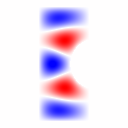
\includegraphics[width=0.093\linewidth]{f/marimba_v07.png} &
	
\includegraphics[width=0.093\linewidth]{f/marimba_v08.png} &
	
\includegraphics[width=0.093\linewidth]{f/marimba_v09.png} \\
	$1\!\!1_\Omega$  & $W$ &
	$\lambda_1$ &
	$\lambda_2$ &
	$\lambda_3$ &
	$\lambda_4$ &
	$\lambda_5$ &
	$\lambda_6$ &
	$\lambda_7$ &
	$\lambda_8$ &
	$\lambda_9$
\end{tabular}

On va résoudre ce problème par force brute, minimisant
fonction~$W\mapsto\left\|\mathrm{sp}_\mathbf{R}\left(B^TWB\right)-\Sigma\right\|^2$
avec des méthode d'optimisation modernes; notamment celles utilisées
en~\emph{deep-learning}, pour lesquelles ce problème est d'une taille
considérée petite.  Pour cela, il faut une implémentation de la
fonction~$A\mapsto\mathrm{sp}_\mathbf R(A)$ que l'optimiseur puisse dériver
localement.  C'est ici qu'il y aura la plupart du travail du stage, qui
pourrait parfaitement être titré~\emph{``a differentiable implementaion of the
eigenvalues computation''}.

Si le stage amène à une conclusion positive, on pourra soumettre une
publication (première!) sur l'application des méthodes de deep learning à la
modélisation d'instruments musicaux.




%Que se serait-il passé si on n'avait découvert les séries de Fourier qu'en 2018
%?  Certainement, on connaitrait la formule de représentation~$f(x)=\sum_{n}
%A_ne^{inx}$, mais probablement pas la formule d'analyse~$\displaystyle
%A_n=\frac1{2\pi}\int_0^{2\pi} f(x)e^{-inx}\mathrm{d}x$.  En effet, la formule
%d'analyse n'est pas vraiment nécessaire en pratique: si l'on peut évaluer la
%fonction~$f(x)$ sur une base de données de millions de points~$(x_i,f_i)$,
%alors on peut retrouver les poids~$A_n$ qui minimisent une~\emph{fonction de
%perte} sur la base de données, par exemple
%$E(A)=\sum_i\left|f(x_i)-f_i\right|^p$.  Les méthodes d'optimisation modernes
%permettent de retrouver facilement les coefficients optimaux~$A_n$ dans ce
%cadre.
%%Pour~$p=2$, on sait
%
%Évidemment, cette description est caricaturale.  Mais aujourd'hui, nous sommes
%exactement dans la même situation avec les réseaux de neurones.  On sait bien
%que beaucoup de fonctions~$f:\mathbf{R}\to\mathbf{R}$ admettent une
%représentation de la forme
%\[
%%	f(x)\approx\left|\cdots\left|A_2\left|A_1\vec
%%	x+b_1\right|+b_2\right|+\cdots +b_N\right|
%	f(x)\approx\rho\!\left(\cdots\rho\!\left(A_2\,\rho\!\left(A_1\vec
%	x+b_1\right)+b_2\right)+\cdots +b_N\right)_1
%\]
%où~$\vec x=(x,\ldots,x)\in\mathbf{R}^M$, la fonction~$\rho$ est une
%non-linéarité fixée, et les matrices~$A_i\in\mathcal{M}_{M,M}(\mathbf{R})$ et
%les vecteurs~$b_i\in\mathbf{R}^M$ sont les~\emph{poids} du réseau.  Les
%paramètres~$N$ et~$M$ s'appellent respectivement la~\emph{profondeur} et
%l'\emph{épaisseur} de la représentation, et leur produit~$MN$ est
%le~\emph{nombre de neurones}.  Couramment, on détermine les
%poids~$\left\{A_i,b_i\right\}$ comme ceux qui minimisent une fonction de perte
%sur une base de données d'évaluations préalables de~$f$.  Trouver une
%expression des poids à partir de la fonction~$f$ est un problème ouvert
%extrêmement difficile, très loin d'être résolu avec les méthodes mathématiques
%que l'on connait.
%On sait, par contre, caractériser les espaces de fonctions
%que on peut approcher à un taux donné en termes de la profondeur et
%l'épaisseur.
%, et on ne sait pas faire autrement.


%\begin{figure}[H]
%	\begin{center}
%		\includegraphics[width=0.49\textwidth]{f/sv.png}
%	\end{center}
%    \vspace{-1.5em}
%	\caption{
%		Photographie satellite d'un ensemble de tas de charbon près
%		d'une raffinerie.  L'objectif du stage consiste à faire un
%		programme qui calcule le volume de la réserve à partir d'une
%		image comme celle-ci.
%	}
%\end{figure}

%{\bf Objectif du stage}\\
%L'objectif est d'avancer vers la solution du problème de l'analyse des réseaux
%de neurones.  Plus concrètement, on va étudier sur quels espaces de fonctions
%on peut obtenir des certains taux d'approximation quand~$N$, $M$ ou~$NM$ vont
%vers infini.  Les résultats du type ``à un même nombre de neurones, un réseau
%profond est plus puissant que un réseau épais'' se formalisent donc comme des
%inclusions entre espaces de fonctions.  Pour cela, on va lire en détail les
%travaux récents de Philip Grohs et ses collaborateurs, essayer de reproduire
%numériquement les résultats d'approximation qui s'y décrivent, et si possible
%les généraliser sur des nouvelles directions (par exemple les réseaux
%convolutionnels).
%On définit par exemple l'espace de
%fonctions~$\mathcal{N}^\alpha,p([a,b])$ comme l'ensemble des
%fonctions~$f:[a,b]\to\mathbf{R}$ telles qu'il existe une suite de réseaux de
%neurones~$f_n$ tels que~$\left\|f_n-f\right\|_{L^p([a,b])}


%Au cours du stage, le groupe d'élèves lira les articles clés sur le sujet, qui
%font appel à des connaissances d'algèbre linéaire, calcul différentiel et
%traitement d'images.  Les méthodes numériques proposées seront enfin mises en
%œuvre avec un langage de programmation choisi par les étudiants (\emph{Python,
%Matlab, ou C/C++}).


    \vspace{-1.5em}
\renewcommand{\refname}{\normalsize Références}
%
\begin{thebibliography}{99}
\vspace{-1em}
{\scriptsize
\bibitem{drum}
	Kac, M..
	{\it Can one hear the shape of a drum?}
	The american mathematical monthly, (1966)

\bibitem{bells}
	McLachlan, N. et al.
	%, Nigjeh, B. K., & Hasell, A. (2003).
	{\it The design of bells with harmonic overtones.}
	The Journal of the Acoustical Society of America, (2003).

\bibitem{mallets}
	Henrique, L. L. et al.
	%, & Antunes, J. (2003).
	{\it Optimal design and physical modelling of mallet percussion
	instruments.}
	Acta Acustica (2003).

\bibitem{inverse}
	Chu, M., \& Golub, G.
	{\it Inverse eigenvalue problems: theory, algorithms, and
	applications}, OUP (2005)

\bibitem{timbre}
	Sethares, W. A.
	{\it Tuning, timbre, spectrum, scale}
	Springer (2005)

\bibitem{clarinet}
	Noreland, D.  et al.
	%, Kergomard, J., Laloë, F., Vergez, C., Guillemain, P., \& Guilloteau, A.
	{\it The logical clarinet: numerical optimization
	of the geometry of woodwind instruments.}
	Acta Acustica (2013)

\bibitem{zoolophone}
	Bharaj, Gaurav, et al.
	{\it Computational design of metallophone contact sounds.}
	SIGGRAPH (2015)

\bibitem{isospectralization}
	Cosmo, Luca, et al. 
	{\it Isospectralization, or how to hear shape, style, and
	correspondence.}
	CVPR (2019)

%\bibitem{perekrestenko}
%	D.~Perekrestenko, P.~Grohs, D.~Elbrächter, H.~Bölcskei,
%	{\it The Universal Approximation Power of Finite-Wdith Deep ReLU
%	Networks},
%	\url{https://arxiv.org/abs/1806.01528},
%	preprint 2018
%
%\bibitem{yarotsky17}
%	Yarotsky,~D.
%	{\it Error bounds for approximations with deep ReLU networks},
%	Neural Networks 94 (2017),
%	\url{http://dx.doi.org/10.1016/j.neunet.2017.07.002}
%
%\bibitem{bolcskei}
%	H.~Bölcskei, P.~Grohs, G.~Kutyniok, P.~Petersen,
%	{\it Optimal Approximation with Sparsely Connected Deep Neural
%	Networks},
%	\url{http://mat.univie.ac.at/~grohs/files/NNapprox.pdf},
%	preprint 2017
%
%%	TODO: add intermediate references
%
%\bibitem{mhaskar}
%	H.N.~Mhaskar,
%	{\it Neural networks for optimal approximation of smooth analytic
%	functions}, 1996
%
%\bibitem{barron}
%	A.R.~Barron,
%	{\it Universal approximation bounds for superposition of a sigmoidal
%	function},
%	IEEE Trans. Inf. Th. 1993
%
%
%\bibitem{hornik}
%	K.~Hornik, M~.Stinchcombe, H.~White,
%	{\it Multilayer feedforward networks are universal approximators},
%	\url{https://doi.org/10.1016/0893-6080(89)90020-8}
%	Neural Networks, 1989
%
%\bibitem{cybenko}
%	G.~Cybenko,
%	{\it Approximations by superpositions of sigmoidal functions},
%	\url{https://doi.org/10.1007\%2FBF02551274}
%	Mathematics of Control, Signals and Systems, 1989


%\bibitem{retinex} Land, E. H., and McCann, J. J. Lightness and Retinex Theory. Journal of the Optical Society of America, 1971.
%
%\bibitem{shepard} Shepard, D. A two-dimensional interpolation function for irregularly-spaced data. ACM national conference, 1968.
%
%%\bibitem{ssao} Bavoil, L. and Sainz, M.. Screen space ambient occlusion. NVIDIA developer information, 6, 2008.
%
%\bibitem{unser} Q. Sun, and M. Unser. Left-inverses of fractional Laplacian and sparse stochastic processes. Advances in Computational Mathematics, 2012.
%
%%\bibitem{whitening} Goldstein, A., and Fattal, R. Blur-Kernel Estimation from Spectral Irregularities. In Computer Vision – ECCV 2012, (2012).
}
\end{thebibliography}

%{\bf old seamless cloning text}
%
%\noindent  \emph{Seamless image cloning} (copier-et-coller sans couture) est un outil important pour l'édition d'images et video
%qui consiste à copier un morceau d'une image source et le coller dans une image de destination de sorte de pas introduire 
%des artefacts visibles sur la frontière de la région modifiée.
%Le renommée méthode de \emph{poisson editing} (Perez et al. 2003) propose de résoudre ce problème
%par la minimisation d'une énergie définie sur le domaine à éditer $\Omega$ (de forme arbitraire)
% \[  \min_{f} \int_{\Omega} | \nabla f  - \mathbf{v} |^2  \mbox{    s.t.    }    f|_{\partial \Omega} = f^*|_{\partial \Omega},\] 
% où $f^*$ denote l'image cible et $\mathbf v$ sont des gradients obtenus a partir de l'image source $g$.
%%
%Lorsque $ \mathbf v = \nabla g$, la solution au problème de poisson editing peut être décrit en termes de
%la solution de l'équation de Laplace sur le domaine $ \Omega $ avec conditions de Dirichlet aux bords.
%Au cours \emph {d'Analyse Hilbertienne et de Fourier} nous avons vu que si le domaine est rectangulaire
%la solution a cette problème peut être calculée efficacement en utilisant la transformée de Fourier rapide.
%Par contre les algorithmes de résolution itératives utilises pour des domaines arbitraires sont généralement lents.
%
%La méthode de \emph{``convolution pyramids''}  récemment proposée  par Farbman et al. (2011) utilise un approche multi-échelle pour calculer des solutions approximatives de l'équation de Laplace de façon très efficace.
%Mais, même si l'algorithme est  simple dans la pratique, les auteurs reconnaissent que son comportement n'est pas entièrement comprise d'un point de vue théorique. 
%
%
%L'objective de cet stage est donc d'étudier l'algorithme de \emph{``convolution pyramids''} appliquée à la resolution de l'équation de Laplace avec conditions de Dirichlet aux bords, pour 
%%comprendre son fonctionnement, 
%identifier ses limites, et éventuellement caracteriser les circonstances dans lesquelles l'approximation obtenue est la pire.
%%Spécifiquement  nous sommes intéressés à la caractérisation des circonstances dans lesquelles l'approximation est la pire.
%Ceci demande réflexion et expérimentation. Durant le stage, le groupe d’élèves lira les articles clés sur le sujer qui leur seront fournis, et qui font appel à des connaissances d’analyse fonctionnelle, calcul variationel, et à pas mal d’effort de programation. \\
%
%%Ce que entraînera lire les principaux articles sur le sujet de  d'interpolation 
%% Pour \c ca il faudra maîtriser la theorie d'analyse multi... ce qui 
%% et à pas mal d’effort de programation. 
% 
%
%%\medskip
%\thispagestyle{empty}
%
%\noindent Burt and E. Adelson,``The laplacian pyramid as a compact image code'' Communications, IEEE Transactions on, vol. 31, no. 4, pp. 532-540, Apr. 1983.\\
%
%\noindent Z. Farbman, R. Fattal, and D. Lischinski,``Convolution pyramids'' ACM Trans. Graph., vol. 30, no. 6, Dec. 2011.\\
%
%\noindent P. Pérez, M. Gangnet, and A. Blake,``Poisson image editing'', ACM Trans. Graph., vol. 22, no. 3, pp. 313-318, Jul. 2003.\\
%
%\noindent D. Shepard, ``A two-dimensional interpolation function for irregularly-spaced data'', in Proceedings of the 1968 23rd ACM national conference, ser. ACM '68., 1968, pp. 517-524. \\
%
%%\noindent S. Darabi, E. Shechtman, C. Barnes, D. B. Goldman, and P. Sen, "Image Melding: Combining Inconsistent Images using Patch-based Synthesis," ACM Transactions on Graphics (TOG) (Proceedings of SIGGRAPH 2012), vol. 31, no. 4, 2012.
%
%%\noindent P. Bhat, B. Curless, M. Cohen, and Zitnick, "Fourier analysis of the 2D screened poisson equation for gradient domain problems," in Computer Vision – ECCV 2008, ser. Lecture Notes in Computer Science,  Springer Berlin Heidelberg, 2008, vol. 5303, pp. 114-128. 


\end{document}  



\newpage

{\bf Gabriele's references don't delete yet: 

\url{https://en.wikipedia.org/wiki/Cauchy_distribution}

\url{http://mathworld.wolfram.com/CauchyDistribution.html}

\url{http://www.math.uah.edu/stat/special/Cauchy.html}

}
\medskip

\newpage

\begin{verbatim}
PROGRAMME DU STAGE
==================

1. Montrer que k(x,y)=(x^2+y^2)^(-1/2) est une fonction localement intégrable.

2. Montrer que si f est localement intégrable et g est à support compact, alors
on peut définire la convolution f*g, qui est une fonction continue.

3. Montrer que \Delta k = k^3 - \delta/2pi au sens des distributions

4. Rappeler la définition de transformée de Fourier d'une distribution
temperée.  Montrer que k est une distribution temperée et montrer que F(k)=k.

5. Montrer que -k*k* = \Delta^{-1}

6. Soit Z_t l'opérateur de zoom de facteur t, défini par Z_t(f)(x)=f(x/t).
Trouver une rélation de commutativité entre Z et k.  La comparer avec la
rélation correspondante pour un noyau Gaussien de taille \sigma.

7. Proposer différentes discretisations de l'opérateur k* sur images carrées.
Certaines de ces discretisation nécéssitent des paramètrees qui seront fixées
plus tard.

8. Implementer chaque une de ces discretisations en C, matlab ou python.

9. Faire des expériences numériques pour vérifier les proprietés formelles de
l'opérateur dans le cas continu.  Optimiser les paramètres des discretisations
afin que les propriétés souhaitées soient le plus exactes possible.

10. Faire des expériences pour illustrer l'importance des opérateurs k et
\Delta k en traitement d'images : retinex, ssao, shephard interpolation,
éditeur de Poisson.

11. Investiguer quel est le temps de calcul optimal en FPS qu'on pourrait
atteindre sur une séquence de vidéo HD (1920x1080) et 4K (4096x2160) en
utilisant FFTW3 sur CPU ou une implementation de FFT en GPU.

12. Lire l'article "convolutional pyramids".  Est-il possible/judicieux
d'implementer cette méthode pour approximer le calcul de l'opérateur k* ?  Quel
serait le temps d'exécution en FPS qu'on pourrait atteindre en CPU et GPU si on
la faisait ?

13. Proposer une implementation rapide de k* selon l'article "convolutional
pyramids".  Combien de coéfficients des filtres restent-t-ils à detérminer ?
Comment pourrait-on *apprendre* ces coéfficients ?

14. Concevoir un plan d'expériences pour apprendre les coéfficients optimaux
des filtres.

15. Implémenter et exécuter ces expériences pour obtenir les coéfficients des
filtres.

16. Implémenter la méthode de calcul de k* résultant.  Évaluer sa performance
visuellement, numériquement, ainsi que sa vitesse en FPS.
\end{verbatim}


\end{document}  


% vim:set tw=79 spell spelllang=fr:
